\documentclass{beamer-custom}
\usepackage{beamer-custom}

\usefonttheme{serif}
% Theme
\usetheme{Montpellier}
\usecolortheme{beaver}
\useinnertheme{circles}

% Navigation
\setbeamertemplate{navigation symbols}{}
\setbeamertemplate{footline}[frame number]

% Frame title formatting
\setbeamertemplate{frametitle}{
    \vspace{0.5em}
    \insertframetitle
    \par
}
%\usepackage{cmbright,bbold}
%\renewcommand{\mathcal}{\mathtt}
\usepackage{kpfonts}
\AtBeginSection[]
{
  \begin{frame}
    \frametitle{Contents}
    \tableofcontents[currentsection]
  \end{frame}
}
% Title page
\title{Amenability: A (Somewhat) Brief Introduction}
\author{Avinash Iyer}
\institute{Occidental College}
\date{March 20, 2025}

\begin{document}
\begin{frame}
    \titlepage
\end{frame}

\begin{frame}{Outline}
    \tableofcontents
\end{frame}
\section{Definitions}%
\begin{frame}
  \frametitle{Groups}
  If $A$ is a set, and $\star\colon A\times A \rightarrow A$ is an operation such that
  \begin{itemize}
    \item $a\star\left(b\star c\right) = \left(a\star b\right)\star c$;
    \item there exists $e_A$ such that $a\star e_A = e_A\star a = a$;
    \item for each $a$ there exists $a^{-1}$ such that $a\star a^{-1} = a^{-1}\star a = e_A$,
  \end{itemize}
  then we call the pair $\left(A,\star\right)$ a \textit{group}.\pause\hfill\break

  We abbreviate $a\star b$ as $ab$.
\end{frame}
\begin{frame}
  \frametitle{Subgroups, Quotient Groups}
  Let $G$ be a group.
  \begin{itemize}
    \item If $H\subseteq G$ is a subset that satisfies, for all $a,b\in H$, $ab^{-1}\in H$, then we say $H$ is a \textit{subgroup}.\pause
    \item If $N\subseteq G$ is a subgroup that satisfies, for all $g\in G$ and $h\in N$, $ghg^{-1}\in N$, then we say $N$ is a \textit{normal subgroup}.\pause
    \item The equivalence classes under the relation $g\sim_{N} g'$ if $g^{-1}g' \in N$ form a group $gN\coloneqq \left[ g \right]_{\sim}$ known as the \textit{quotient group} $G/N$.
  \end{itemize}
\end{frame}
\begin{frame}
  \frametitle{Some Groups}
  \begin{itemize}
    \item The integers $\Z$ are a group under addition.
    \item The group of invertible $n\times n$ matrices over $\C$, $\text{GL}_{n}\left(\C\right)$, is a group under matrix multiplication.
    \item The subgroup $\text{SO}(n)\subseteq \text{GL}_{n}\left( \R \right)$ consisting of $n\times n$ orthogonal matrices with determinant $1$ is a group under multiplication.
  \end{itemize}
\end{frame}
\begin{frame}
  \frametitle{Group Actions}
  Let $G$ be a group, and $X$ a set. Let $\rho\colon G\times X \rightarrow X$ be a function that satisfies, for all $g,h\in G$ and $x\in X$,
  \begin{itemize}
    \item $\rho\left( e_G, x\right) = x$;
    \item $\rho\left( g,\rho\left( h,x \right) \right) = \rho\left( gh,x \right)$.
  \end{itemize}
  Then, we say $\rho$ is an \textit{action} of $G$ on $X$. We write $\rho\left( g,x \right) = g\cdot x$.
\end{frame}
\begin{frame}
  \frametitle{$\sigma$-Algebras and Measures}
  If $X$ is a set, then a collection of subsets $\set{A_{i}}_{i\in I} = \mathcal{A}\subseteq P(X)$ is known as an \textit{algebra} of subsets if
  \begin{enumerate}
    \item $\emptyset,X\in \mathcal{A}$;
    \item for any $A_i\in \mathcal{A}$, $A_i^{c}\in \mathcal{A}$;
    \item for any $A_i,A_j\in \mathcal{A}$, $A_i\cup A_j\in \mathcal{A}$.
  \end{enumerate}\pause
  If, for any countable collection, $\set{A_n}_{n\geq 1}\subseteq \mathcal{A}$, condition (3) holds, then we say $\mathcal{A}$ is a \textit{$\sigma$-algebra} of subsets.
\end{frame}
\begin{frame}
  \frametitle{$\sigma$-Algebras and Measures, Cont'd}
  If $X$ is a set and $\mathcal{A}$ is a $\sigma$-algebra, then a map $\mu\colon \mathcal{A}\rightarrow [0,\infty]$ that satisfies:
  \begin{itemize}
    \item $\mu\left( \emptyset \right) = 0$;
    \item for disjoint sets $A,B\in \mathcal{A}$, $\mu\left( A\sqcup B \right) = \mu\left( A \right) + \mu\left( B \right)$,
  \end{itemize}
  then we say $\mu$ is a \textit{finitely additive} measure.\pause \newline

  If $\set{A_n}_{n\geq 1}$ is a countable collection of disjoint sets, then if $\mu$ satisfies
  \begin{itemize}
    \item $\displaystyle \mu\left( \bigcup_{n\geq 1}A_n \right) = \sum_{n\geq 1}\mu\left( A_n \right)$,
  \end{itemize}
  we say $\mu$ is a measure. If $\mu\left( X \right) = 1$, then we say $\mu$ is a probability measure.
\end{frame}
\section{Paradoxical Decompositions}%
\begin{frame}
  \frametitle{Questions?}
  \begin{itemize}
    \item If $G$ is a group, is it possible to reconstruct $G$ by using some subset of $G$?
    \item When may we find a finitely additive probability measure $\mu\colon P(G)\rightarrow [0,1]$ such that $\mu\left( E \right) = \mu\left( tE \right)$ for all $E\subseteq G$?
    \item Are these questions even related?
  \end{itemize}
\end{frame}
\begin{frame}
  \frametitle{Free Groups}
  \begin{itemize}
    \item We begin by considering a special group, known as $F(a,b)$ or the \textit{free group on two generators}.\pause
    \item We define $F(a,b)$ to be the set of all ``words'' in the alphabet $\set{a,b,a^{-1},b^{-1}}$, subject to the condition that, for $w,w'\in F(a,b)$,
      \begin{align*}
        waa^{-1}w' \sim wa^{-1}aw' \sim ww'\\
        wbb^{-1}w' \sim wb^{-1}bw' \sim ww'.
      \end{align*}
    \item Examples: $a^2bab^{-1},b^{-1}a^2b^2ab\in F(a,b)$.
  \end{itemize}
\end{frame}
\begin{frame}
  \frametitle{A Curiosity}
  Let $W(b)\subseteq F(a,b)$ be all the words that start with $b$. Then, $b^{-1}W(b)$ consists of \pause
  \begin{itemize}
    \item all words that start with $a$;
    \item all words that start with $a^{-1}$;
    \item all words that start with $b$ --- think words that start with $b^2$ before you multiply $b^{-1}$.\pause
  \end{itemize}
  Thus, all we need to do is add back $W\left( b^{-1} \right)$ to get $F(a,b)$ back.
  \begin{align*}
    F(a,b) &= W\left( b^{-1} \right)\cup b^{-1}W(b).
  \end{align*}\pause
\end{frame}
\begin{frame}
  \frametitle{A Curiosity, Cont'd}
  Similarly, we can do this for $a$, giving a decomposition of $F(a,b)$ in two separate ways:
  \begin{align*}
    F(a,b) &= b^{-1}W(b)\cup W\left( b^{-1} \right)\\
           &= a^{-1}W(a)\cup W\left( a^{-1} \right).
  \end{align*}\pause
  Furthermore, note that $W\left( a \right),W\left( b \right),W\left( a^{-1} \right),W\left( b^{-1} \right)$ are disjoint.\pause\newline

  These decompositions seem to be downright paradoxical --- we take a part of the group, translate some of it, and get the whole group back!
\end{frame}
\begin{frame}
  \frametitle{Defining Paradoxical Decompositions}
  Let $G$ be a group. A \textit{paradoxical decomposition} of $G$ consists of
  \begin{itemize}
    \item pairwise disjoint subsets $A_1,\dots,A_n,B_1,\dots,B_m\subseteq G$; and
    \item elements $g_1,\dots,g_n,h_1,\dots,h_m\in G$;
  \end{itemize}
  such that
  \begin{align*}
    G &= \bigcup_{i=1}^{n}g_iA_i\\
      &= \bigcup_{j=1}^{m}h_jB_j.
  \end{align*}\pause
  If $G$ admits a paradoxical decomposition, we say $G$ is \textit{paradoxical}.
\end{frame}
\begin{frame}
  \frametitle{Paradoxical Actions}
  If $G$ acts on a set $X$, then a subset $A\subseteq X$ is \textit{$G$-paradoxical} if there exist
  \begin{itemize}
    \item pairwise disjoint subsets $A_1,\dots,A_n,B_1,\dots,B_m\subseteq A$; and
    \item elements $g_1,\dots,g_n,h_1,\dots,h_m\in G$
  \end{itemize}
  such that
  \begin{align*}
    A &= \bigcup_{i=1}^{n}g_i\cdot A_i\\
      &= \bigcup_{j=1}^{m}h_j\cdot B_j.
  \end{align*}\pause
  A paradoxical group is a paradoxical set under the action of left-multiplication.
\end{frame}
\begin{frame}
  \frametitle{Depiction}
  \begin{center}
    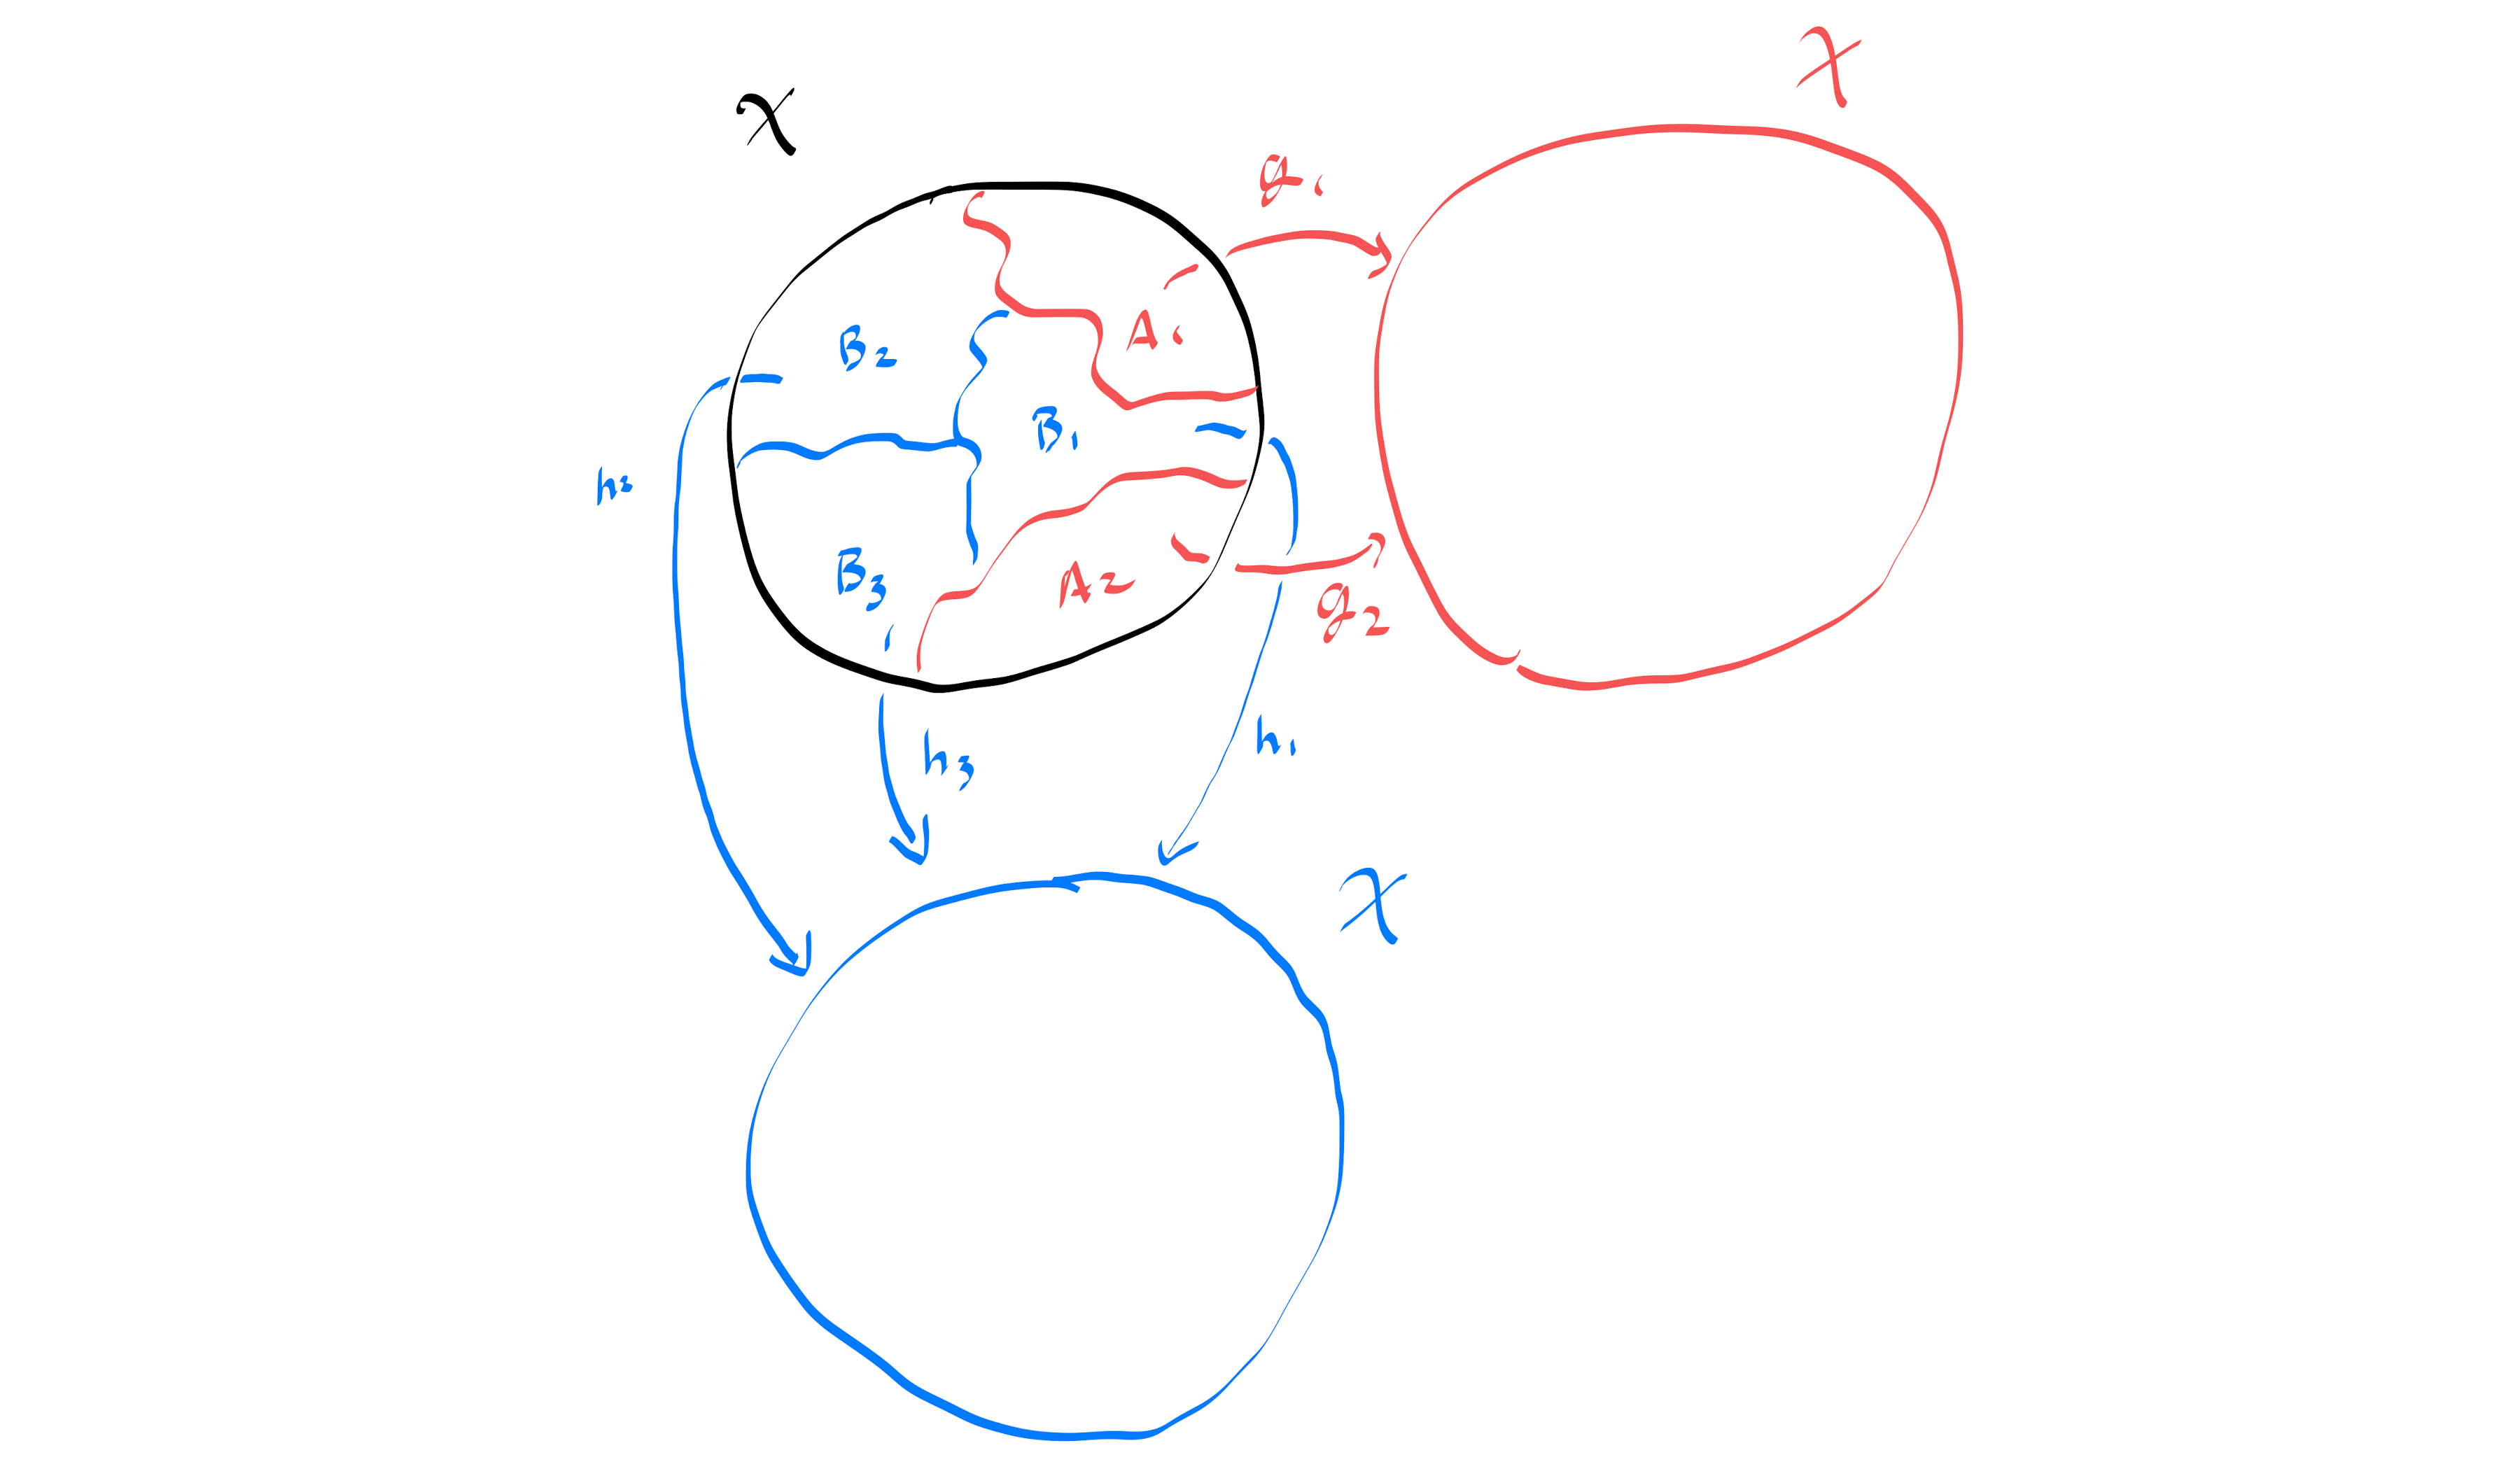
\includegraphics[scale=0.17]{images/paradoxical_decomposition_2.png}
  \end{center}
\end{frame}
\begin{frame}
  \frametitle{Examples}
  \begin{itemize}
    \item The free group $F(a,b)$ is paradoxical.\pause
    \item Any group that contains a paradoxical subgroup is paradoxical.
    \item $F(S)$, where $S$ is any nonempty set with more than two elements, is paradoxical.
  \end{itemize}
\end{frame}
\begin{frame}
  \frametitle{A Paradoxical Subgroup of $\text{SO}(3)$}
  The following two matrices (and their inverses) generate a subgroup of $\text{SO}(3)$ that is isomorphic to $F(a,b)$.
  \begin{align*}
    A &= \begin{pmatrix}3/5 & 4/5 & 0 \\  -4/5 & 3/5 & 0 \\ 0 & 0 & 1\end{pmatrix}\\
    B &= \begin{pmatrix}1 & 0 & 0 \\ 0 & 3/5 & -4/5 \\ 0 & 4/5 & 3/5\end{pmatrix}.
  \end{align*}\pause
  This is proven using the Ping-Pong lemma.
\end{frame}
\begin{frame}
  \frametitle{Introducing the Banach--Tarski Paradox}
  \begin{theorem}[The Banach--Tarski Paradox]
    Let $A$ and $B$ be bounded subsets of $\R^3$ with nonempty interior. There is a partition of $A$ into finitely many disjoint subsets such that a sequence of isometries applied to these subsets yields $B$.
  \end{theorem}\pause
  \begin{itemize}
    \item In other words, not all subsets of $\R^3$ have a definite ``volume'' invariant under isometry.
  \end{itemize}
\end{frame}
\begin{frame}
  \frametitle{Equidecomposability}
  Let $G$ be a group that acts on a set $X$, and let $A,B\subseteq X$. If there exist
  \begin{itemize}
    \item finite partitions, $A_1,\dots,A_n\subseteq A$, $B_1,\dots,B_n\subseteq B$
    \item group elements $g_1,\dots,g_n\in G$
  \end{itemize}
  such that $g_i\cdot A_i = B_i$, then we say $A$ and $B$ are \textit{$G$-equidecomposable}.\pause\newline

  Effectively, $A$ and $B$ are ``equal'' to each other up to the group action.\pause\newline

  If $A$ is $G$-paradoxical, then so too is $B$.
\end{frame}
\begin{frame}[allowframebreaks]
  \frametitle{The Banach--Tarski Paradox: Proof Outline}
  \begin{enumerate}[(1)]
    \item We use the two matrices
      \begin{align*}
        A &= \begin{pmatrix}3/5 & 4/5 & 0 \\  -4/5 & 3/5 & 0 \\ 0 & 0 & 1\end{pmatrix}\\
        B &= \begin{pmatrix}1 & 0 & 0 \\ 0 & 3/5 & -4/5 \\ 0 & 4/5 & 3/5\end{pmatrix}.
      \end{align*}
      to generate a subgroup of $\text{SO}\left( 3 \right)$ isomorphic to $F(a,b)$.
    \item We use the decomposition 
      \begin{align*}
        F\left( a,b \right) &= a^{-1}W\left( a \right)\cup W\left( a^{-1} \right)\\
                            &= b^{-1}W\left( b \right) \cup W\left( b^{-1} \right)
      \end{align*}
      to duplicate the unit sphere in $\R^3$, $S^2$, except for a countable subset $D$. (The \textit{Hausdorff Paradox}.)
    \item We show that $S^2$ and $S^2\setminus D$ are $\text{SO}\left( 3 \right)$-equidecomposable --- there is thus a paradoxical decomposition of $S^2$.
    \item We show that the unit ball, $B\left( 0,1 \right)\subseteq \R^3$, is paradoxical under the isometry group $\text{E}\left( 3 \right)$.
    \item Define a relation $A\preceq B$ if $A$ is $G$-equidecomposable with a subset of $B$, and show that if $A\preceq B$ and $B\preceq A$, then $A$ and $B$ are $G$-equidecomposable.
    \item Show that $A\subseteq \R^3$ is equidecomposable with a subset of $B\subseteq \R^3$.\pause
  \end{enumerate}
  We're done...\pause or are we?
\end{frame}
\section{From Paradoxical Decompositions to Amenability}%
\begin{frame}
  \frametitle{Ill-Behaved Groups}
  \begin{itemize}
    \item The way that our copy of $F(a,b)$ helped ``create'' the Banach--Tarski paradox suggests that $F(a,b)$ is a particularly ill-behaved group.
    \item Let $\nu\colon F(a,b)\rightarrow [0,1]$ be a probability measure --- we will show that $\nu$ \textit{cannot} be translation-invariant (i.e., $\nu\left( tE \right) = \nu\left( E \right)$ for all $t\in F(a,b),E\subseteq F(a,b)$).
  \end{itemize}
\end{frame}
\begin{frame}
  \frametitle{Ill-Behaved Groups, Cont'd}
  Suppose such a translation-invariant $\nu$ exists. Taking
  \begin{align*}
    F(a,b) &= W(a)\sqcup W\left( a^{-1} \right) \sqcup W\left( b \right) \sqcup W\left( b^{-1} \right),
  \end{align*}
  we have
  \begin{align*}
    1 &= \nu\left( W\left( a \right) \right) + \nu\left( W\left( a^{-1} \right) \right) + \nu\left( W\left( b \right) \right) + \nu\left( W\left( b^{-1} \right) \right)\\
      &= \nu\left( a^{-1}W\left( a \right) \right) + \nu\left( W\left( a^{-1} \right) \right) + \nu\left( b^{-1}W\left( b \right) \right) + \nu\left( W\left( b^{-1} \right) \right)\\
      &= \nu\left( a^{-1}W\left( a \right)\sqcup W\left( a^{-1} \right) \right) + \nu\left( b^{-1}W\left( b \right) \sqcup W\left( b^{-1} \right) \right)\\
      &= \nu\left( F(a,b) \right) + \nu\left( F(a,b) \right)\\
      &= 2.
  \end{align*}\pause
  Huh.
\end{frame}
\begin{frame}
  \frametitle{Amenability}
  Let $G$ be a group. A \textit{mean} is a finitely additive probability measure $\nu\colon G\rightarrow [0,1]$ such that
  \begin{align*}
    \nu\left( tE \right) &= \nu\left( E \right)
  \end{align*}
  for all $t\in G$ and $E\subseteq G$.\newline

  If $G$ admits a mean, we say $G$ is \textit{amenable}.
\end{frame}
\begin{frame}
  \frametitle{Examples}
  \begin{itemize}
    \item Finite groups are amenable: let $\delta_t$ be the point mass at $t\in G$,
      \begin{align*}
        \delta_t(s) &= \begin{cases}
          1 & t = s\\
          0 & t\neq s
        \end{cases}.
      \end{align*}
      Then,
      \begin{align*}
        \nu &= \frac{1}{\left\vert G \right\vert} \sum_{t\in G}\delta_t
      \end{align*}
      is a mean.
    \item Abelian (commutative) groups are amenable.
    \item The free group, $F(a,b)$, is \textit{not} amenable.
  \end{itemize}
\end{frame}
\section{Equivalent Definitions and Other Criteria}%
% Følner condition, Cayley graph, talk about intuition behind Følner condition
% Growth, Functional Analysis, Representations, 
\section{Remarks and Acknowledgments}%
\begin{frame}
  \frametitle{Some Recent Developments}
\end{frame}

\end{document}
